\chapter{Funciones del Administrador}\label{cap:administracion}

\disponible Solo Administrador. Estas opciones aparecen en el menú bajo
\textbf{Administración}, y la pestaña \textbf{Asignaciones} dentro de cada
expediente.

% ---------------------------------------------------------------------
\section{Invitar a un integrante}\label{sec:invitar}

\paraque Envía un enlace privado por correo para que la persona cree su
propia cuenta (\cref{sec:aceptar-invitacion}).

\pasos
\begin{enumerate}
  \item En el menú, haga clic en \textbf{Equipo}.
  \item En \textbf{Invitaciones al despacho}, escriba el
        \textbf{Nombre de la persona invitada} y el
        \textbf{Correo de la invitación}.
  \item Elija el \textbf{Rol de la invitación}: \textbf{Asistente legal},
        \textbf{Litigante} o \textbf{Cliente}.
  \item Haga clic en \textbf{Enviar invitación}.
\end{enumerate}

\begin{figure}[H]
  \centering
  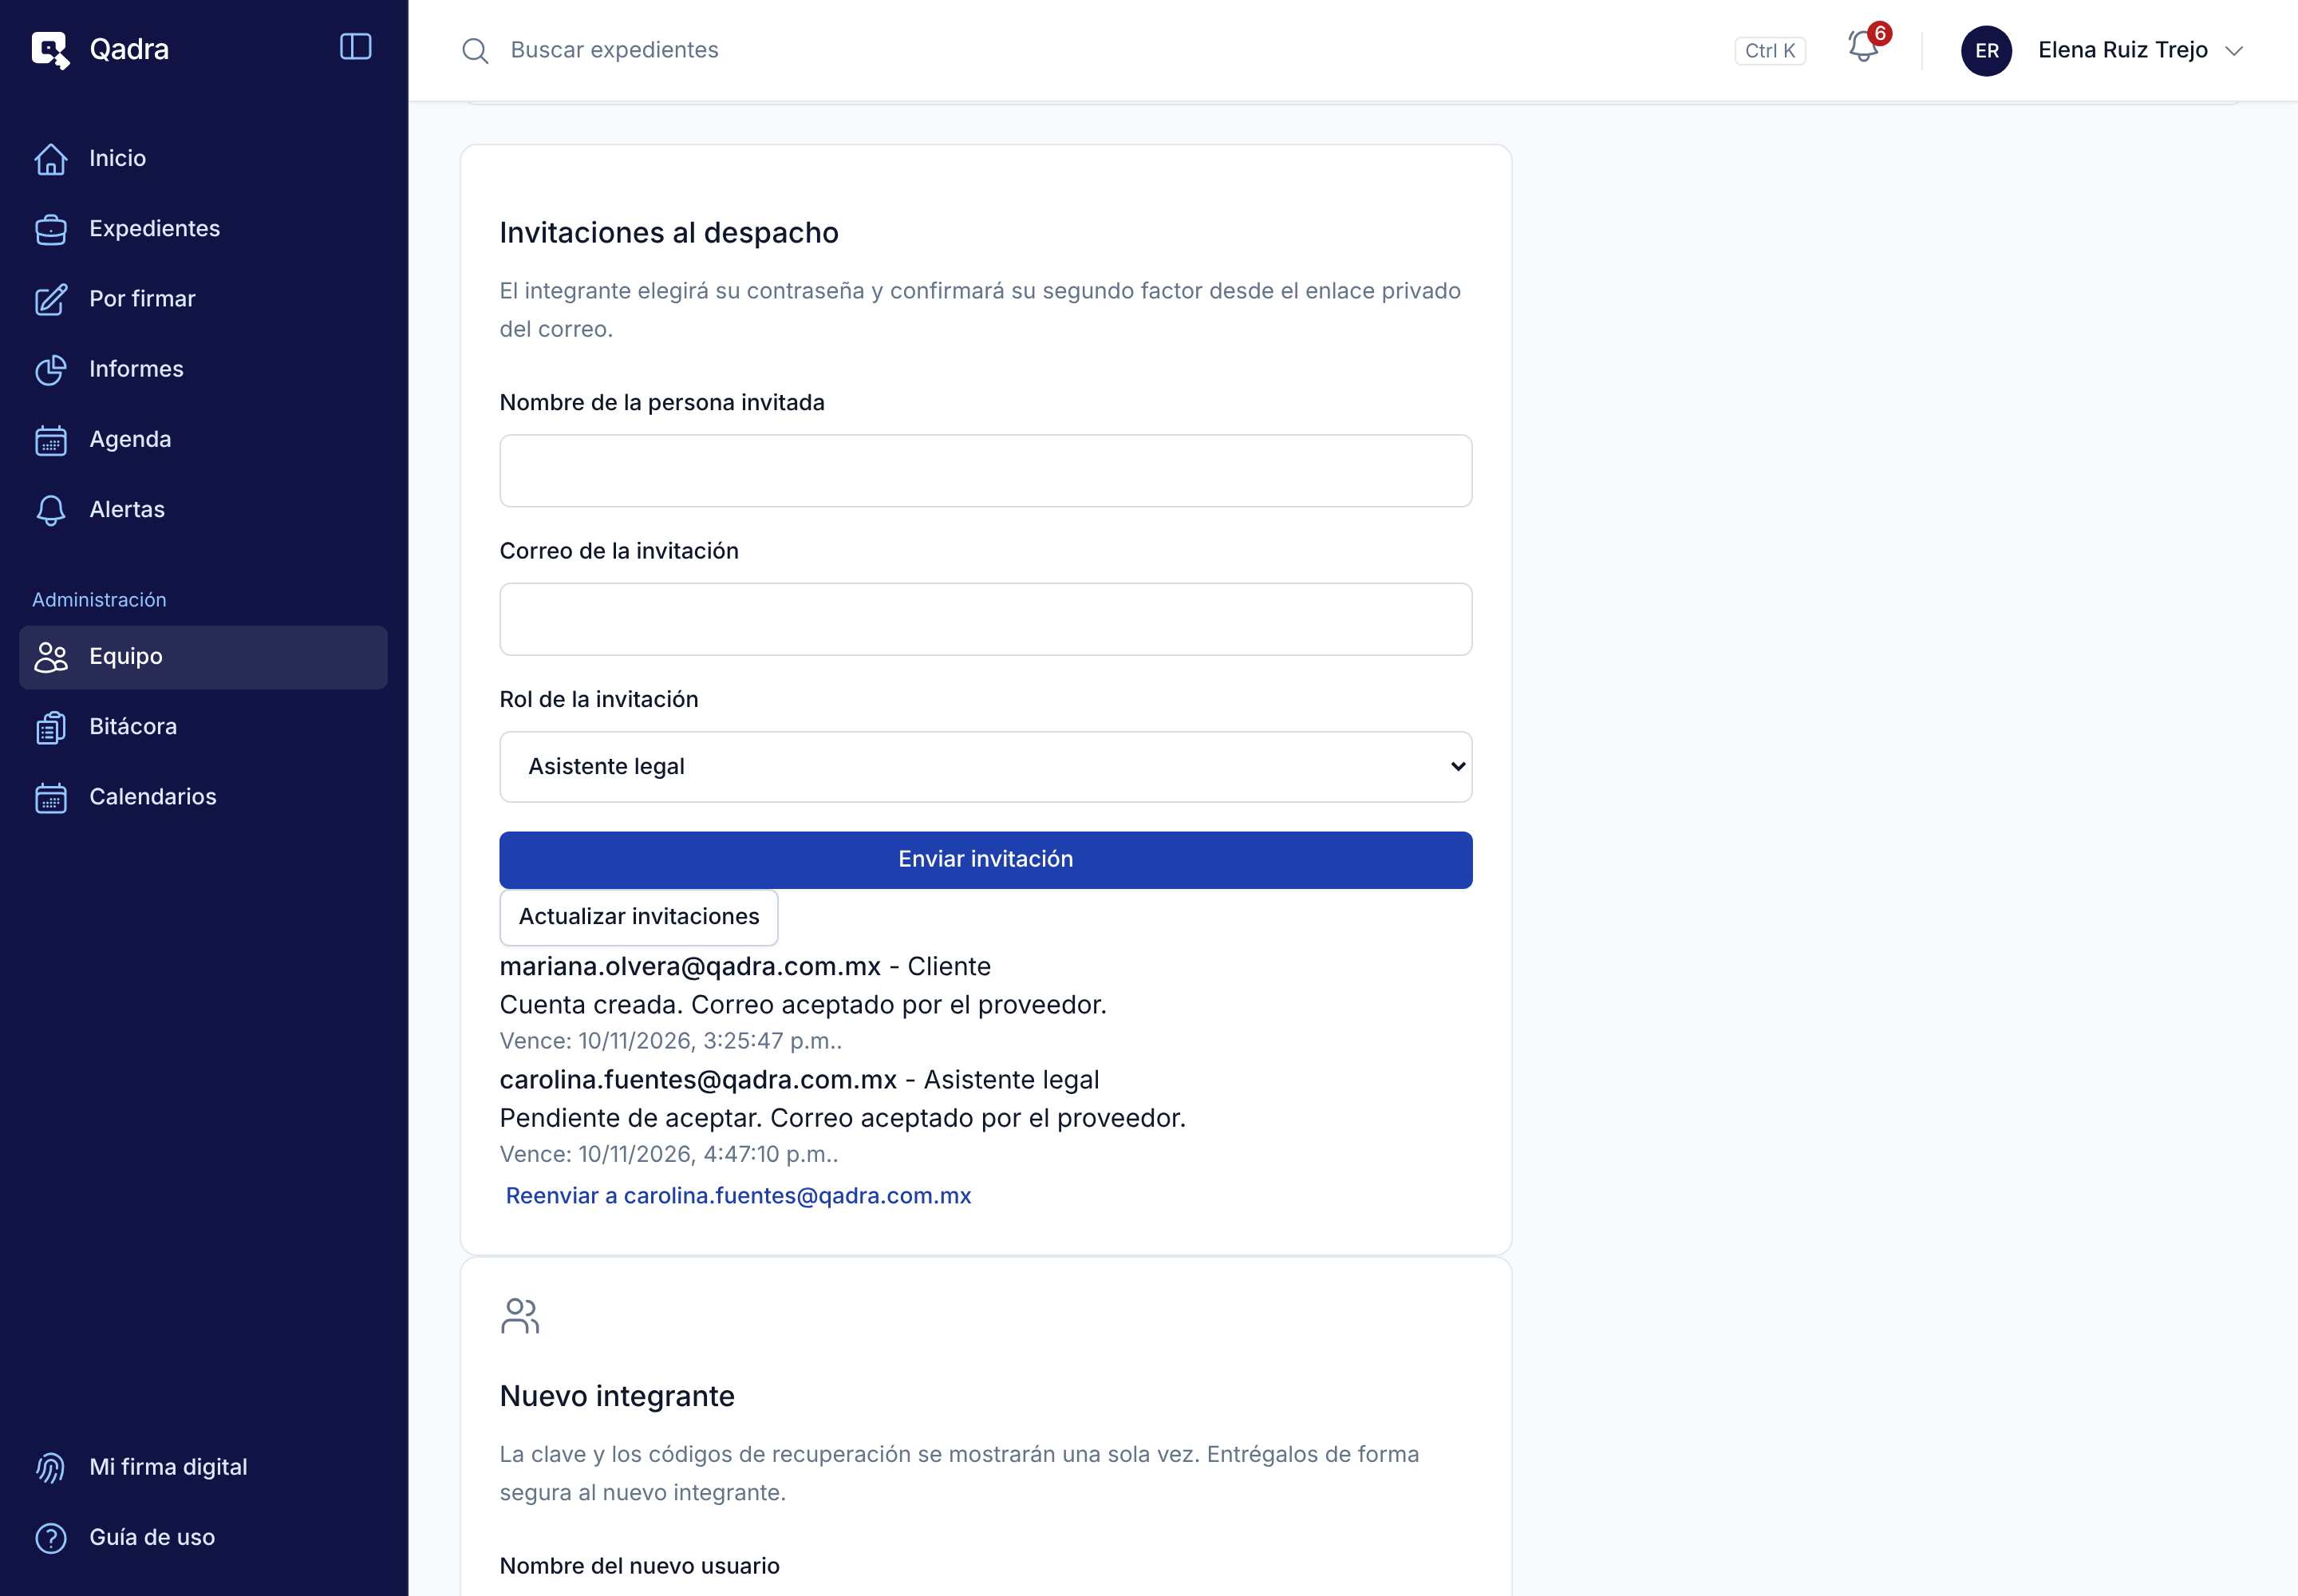
\includegraphics[width=0.9\textwidth]{capturas/A-44-invitaciones.png}
  \caption{Invitaciones al despacho.}
  \label{fig:manual-invitaciones}
\end{figure}

\resultado Aparece \enquote{Invitación registrada para [correo].} y la
invitación se agrega a la lista con su estado y fecha de vencimiento.

\begin{table}[H]
  \centering
  \caption{Estados de una invitación.}\label{tab:estados-invitacion}
  \begin{tabularx}{\textwidth}{L{5.2cm} Y}
    \toprule
    \textbf{Estado} & \textbf{Qué significa} \\
    \midrule
    \textbf{Pendiente de aceptar}        & La persona aún no abre el enlace. \\
    \textbf{Pendiente de confirmar MFA}  & Eligió su contraseña, pero no ha confirmado su segundo factor. \\
    \textbf{Cuenta creada}               & La cuenta ya existe. \\
    \textbf{Enlace vencido o retirado}   & El enlace ya no funciona; reenvíe la invitación. \\
    \bottomrule
  \end{tabularx}
\end{table}

\begin{itemize}
  \item Para enviar un enlace nuevo, haga clic en
        \textbf{Reenviar a [correo]} y luego en \textbf{Confirmar reenvío}.
        El enlace anterior deja de funcionar.
  \item La lista también indica la entrega del correo, por ejemplo
        \textbf{Correo aceptado por el proveedor} o
        \textbf{Correo rechazado}.
\end{itemize}

% ---------------------------------------------------------------------
\section{Dar de alta a un integrante directamente}\label{sec:alta-directa}

\paraque Crea una cuenta sin correo de invitación. También permite crear otro
Administrador.

\pasos
\begin{enumerate}
  \item En \textbf{Equipo}, vaya a \textbf{Nuevo integrante}.
  \item Escriba el \textbf{Nombre del nuevo usuario}, el
        \textbf{Correo del nuevo usuario} y una \textbf{Contraseña inicial}
        de al menos 12 caracteres.
  \item Elija el \textbf{Rol}: \textbf{Asistente legal},
        \textbf{Litigante}, \textbf{Administrador} o \textbf{Cliente}.
  \item Haga clic en \textbf{Crear usuario}. Para abandonar el alta, use
        \textbf{Descartar alta y volver al directorio}.
  \item En \textbf{Configura el segundo factor}, copie la
        \textbf{Clave de configuración} y los
        \textbf{Códigos de recuperación}.
  \item Marque \textbf{Ya guardé la clave y los códigos} y haga clic en
        \textbf{Finalizar}.
\end{enumerate}

\begin{figure}[H]
  \centering
  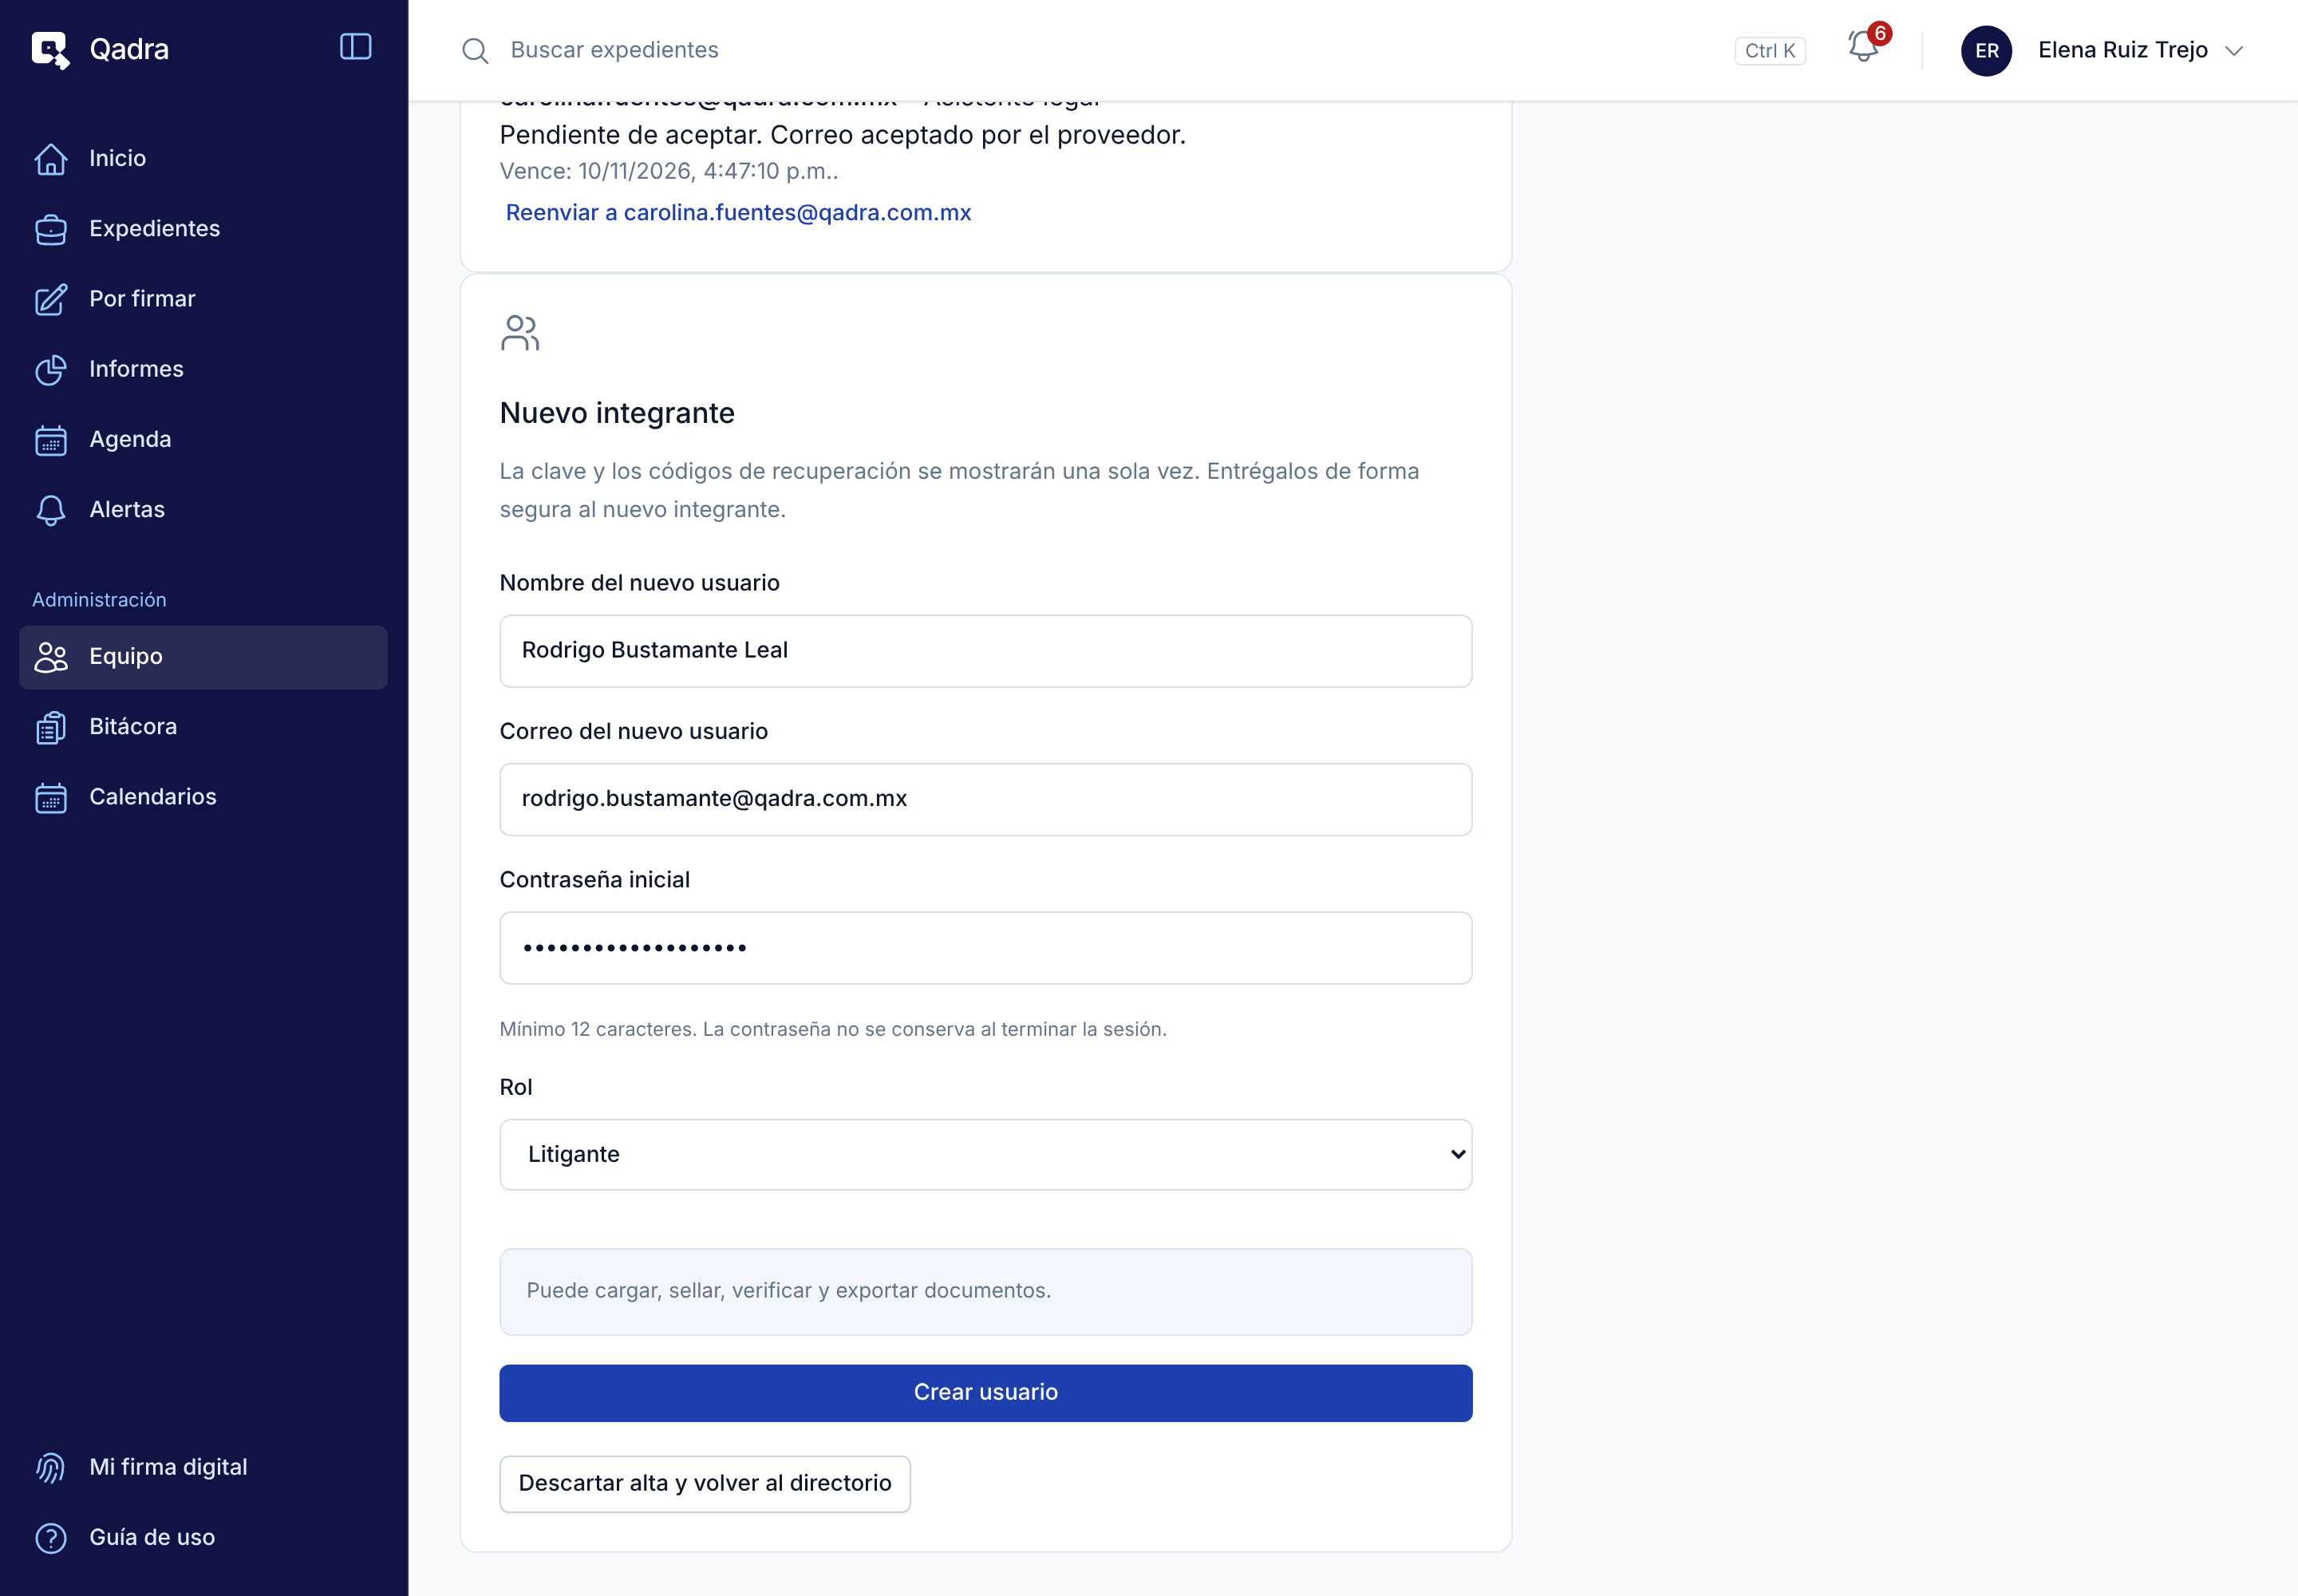
\includegraphics[width=0.9\textwidth]{capturas/A-45-nuevo-integrante.png}
  \caption{Alta directa de un integrante.}
  \label{fig:manual-nuevo-integrante}
\end{figure}

\resultado La cuenta aparece en el \textbf{Directorio de cuentas}.

\importante{La clave y los códigos se muestran una sola vez. Entréguelos al
nuevo integrante por un medio seguro, junto con su contraseña inicial.}

% ---------------------------------------------------------------------
\section{Cambiar el rol o desactivar una cuenta}\label{sec:administrar-acceso}

\paraque Cambia el rol de una cuenta o la desactiva para bloquear su acceso.

\pasos
\begin{enumerate}
  \item En \textbf{Equipo}, vaya a \textbf{Directorio de cuentas}. Si es
        necesario, use \textbf{Buscar por correo}, \textbf{Rol de la cuenta}
        o \textbf{Estado de la cuenta} y haga clic en
        \textbf{Buscar cuentas}.
  \item Haga clic en \textbf{Administrar acceso de [correo]}.
  \item Elija el nuevo \textbf{Rol de la cuenta} o el
        \textbf{Estado de la cuenta} (\textbf{Activa} o \textbf{Inactiva}).
  \item Haga clic en \textbf{Revisar acceso}. En
        \textbf{Confirmar los permisos seleccionados} revise el cambio
        (por ejemplo, \enquote{Asistente legal / Activa a Litigante / Activa.})
        y haga clic en \textbf{Confirmar cambio de acceso}; para corregirlo,
        use \textbf{Editar selección}.
\end{enumerate}

\begin{figure}[H]
  \centering
  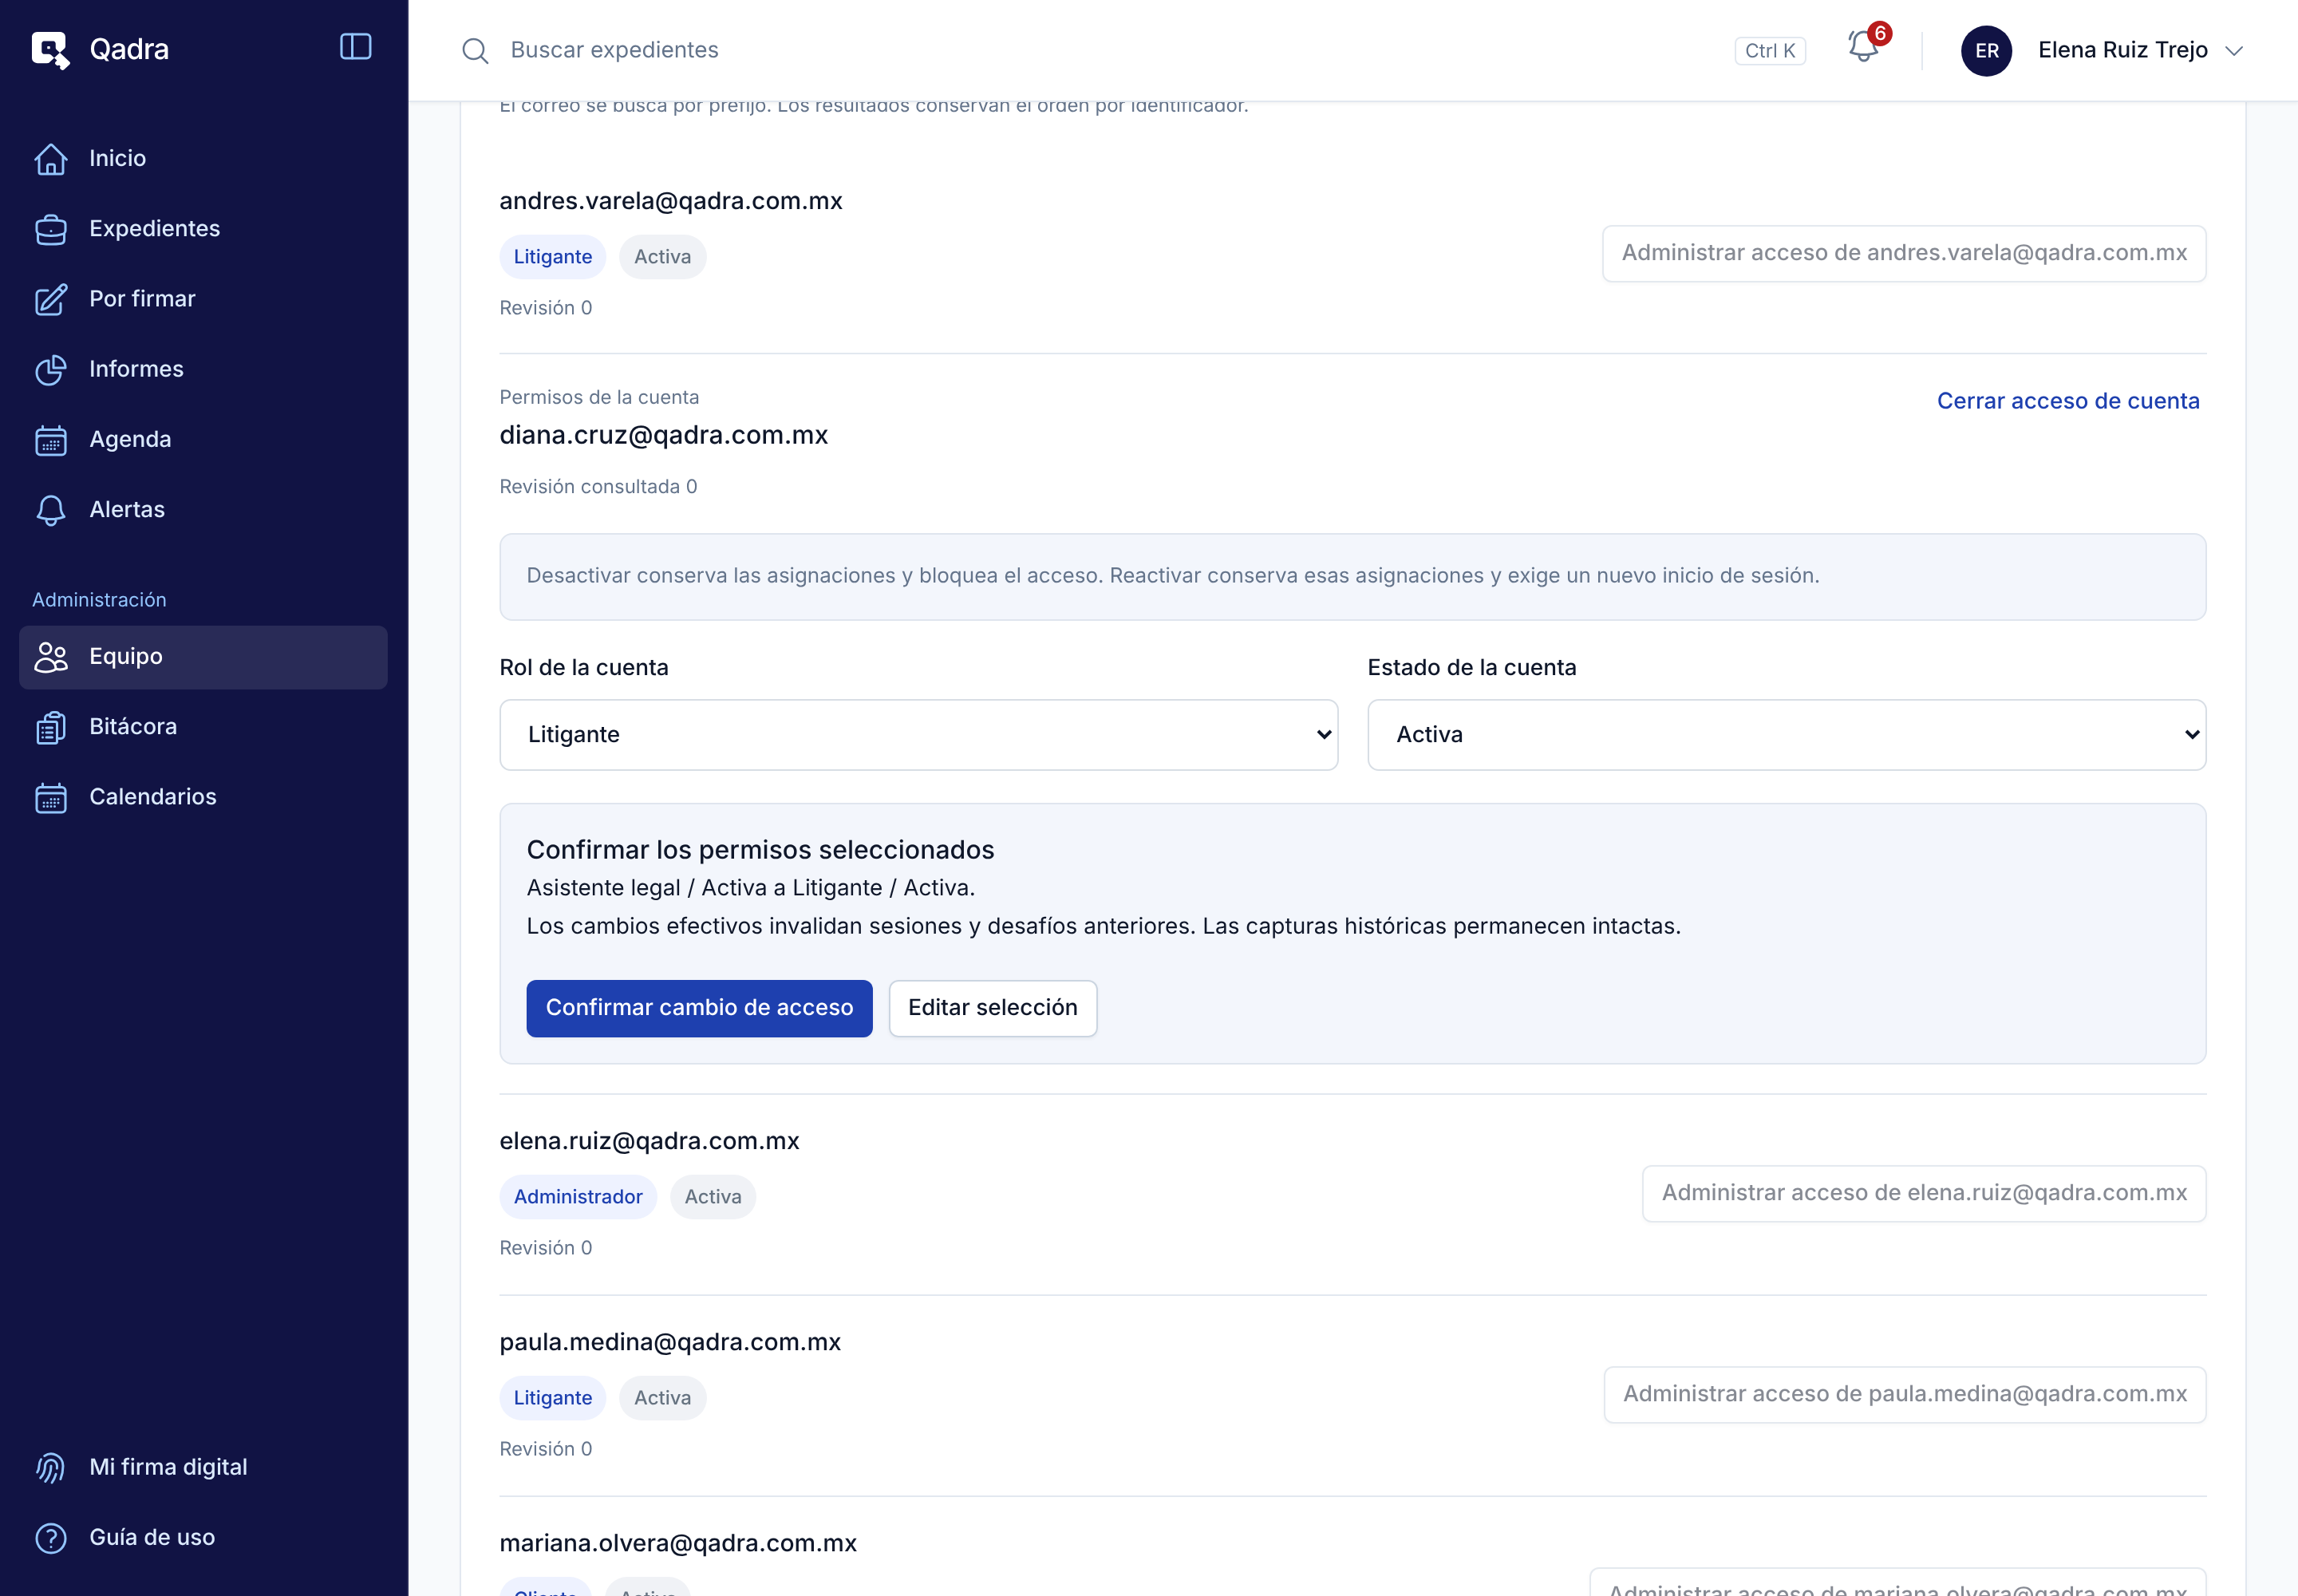
\includegraphics[width=0.9\textwidth]{capturas/A-46-administrar-acceso.png}
  \caption{Cambio de acceso de una cuenta.}
  \label{fig:manual-administrar-acceso}
\end{figure}

\resultado Aparece \enquote{Los permisos de la cuenta se confirmaron.} Las
sesiones anteriores de esa cuenta se cierran.

\begin{itemize}
  \item Desactivar conserva las asignaciones de la cuenta, pero bloquea su
        acceso. Al reactivarla, la persona debe iniciar sesión de nuevo.
  \item \textbf{Cerrar acceso de cuenta} cierra el editor sin cambios.
  \item Siempre debe quedar al menos un Administrador activo; Qadra no
        permite retirar al último.
  \item Si cambia su propio rol o estado, su sesión se cerrará.
\end{itemize}

% ---------------------------------------------------------------------
\section{Asignar cuentas a un expediente}\label{sec:asignaciones}

\paraque Da o retira a un Litigante, Asistente legal o Cliente el acceso a un
expediente.

\pasos
\begin{enumerate}
  \item Abra el expediente y haga clic en la pestaña \textbf{Asignaciones}.
  \item En \textbf{Selección de cuentas}, elija \textbf{Cuentas disponibles}
        (para asignar) o \textbf{Cuentas asignadas} (para retirar). Haga clic
        en \textbf{Buscar asignaciones}.
  \item Haga clic en \textbf{Asignar} o \textbf{Retirar} en la tarjeta de la
        cuenta.
  \item Haga clic en \textbf{Confirmar asignación} o
        \textbf{Confirmar retiro}.
\end{enumerate}

\begin{figure}[H]
  \centering
  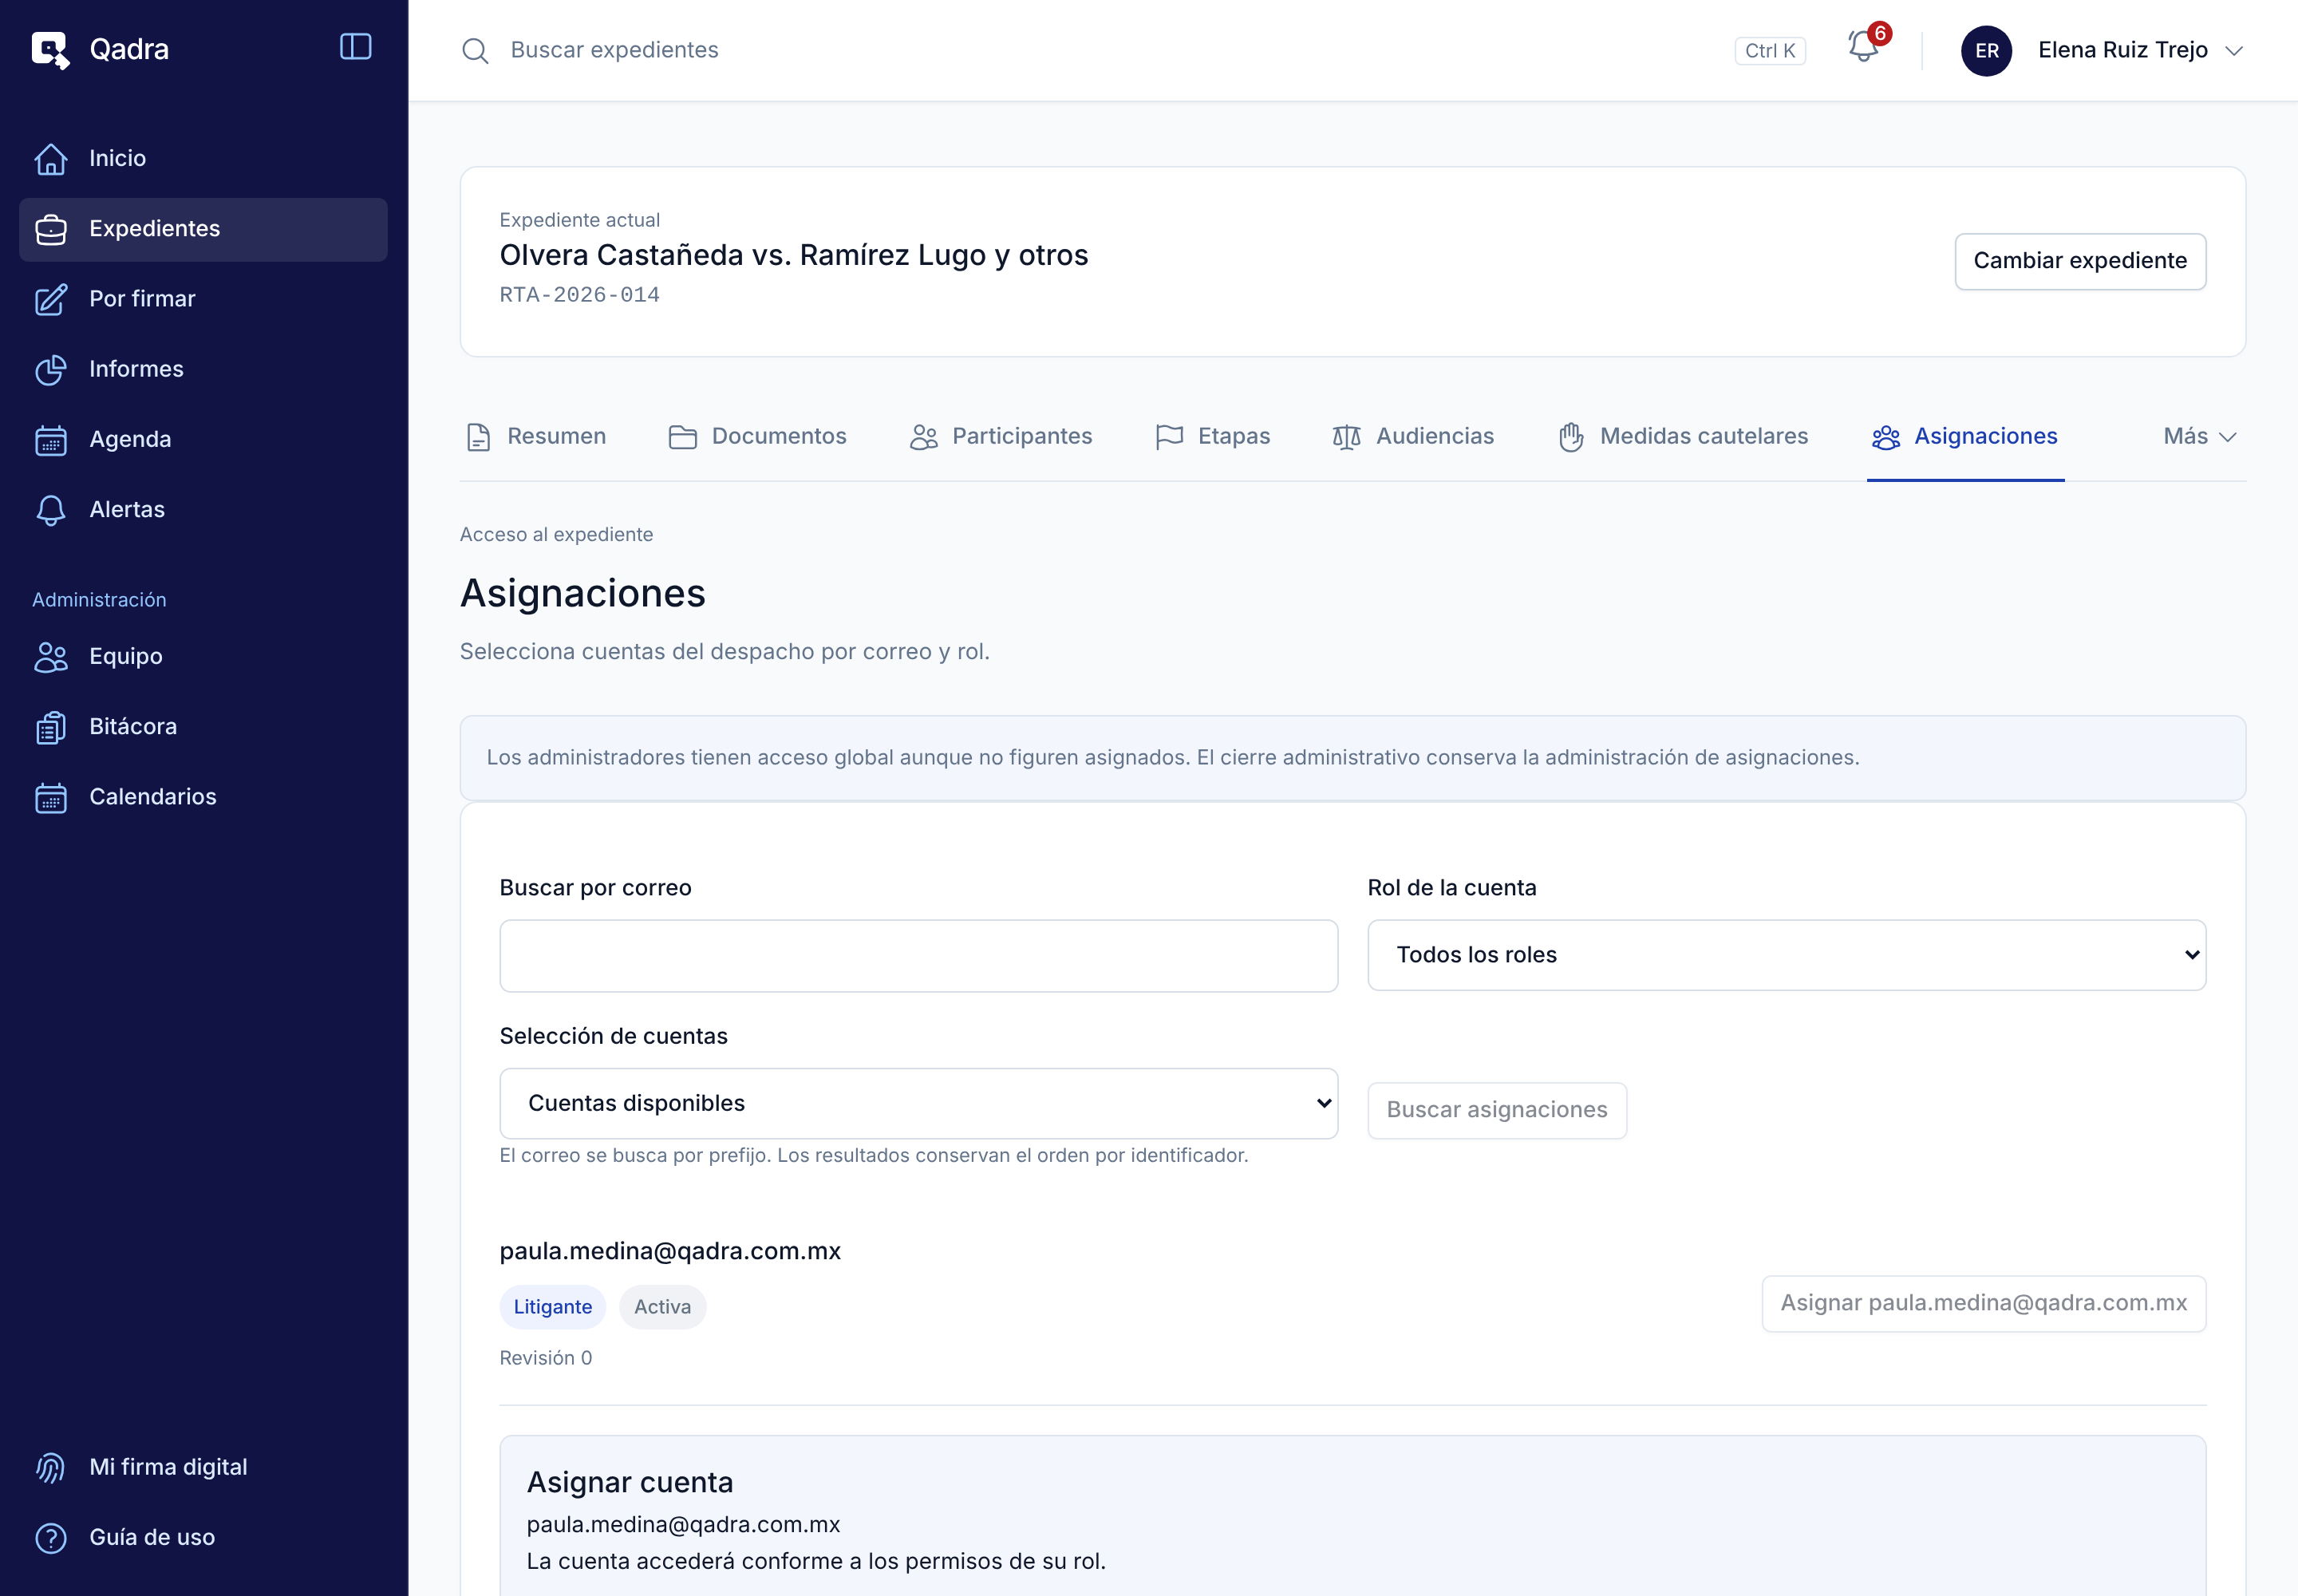
\includegraphics[width=0.9\textwidth]{capturas/A-47-asignaciones.png}
  \caption{Asignación de una cuenta a un expediente.}
  \label{fig:manual-asignaciones}
\end{figure}

\resultado Aparece \enquote{Asignación confirmada.} o \enquote{Retiro de
asignación confirmado.}

\nota{Los Administradores tienen acceso a todos los expedientes aunque no
estén asignados. Retirar una asignación conserva la cuenta y su historial.}

% ---------------------------------------------------------------------
\section{Bitácora e incidentes de integridad}\label{sec:bitacora}

\paraque Muestra los movimientos registrados en el despacho y comprueba que
ninguno se haya alterado o eliminado.

\pasos
\begin{enumerate}
  \item En el menú, haga clic en \textbf{Bitácora}.
  \item En \textbf{Integridad de la cadena}, haga clic en
        \textbf{Verificar cadena}.
  \item En \textbf{Movimientos registrados}, elija el periodo
        (\textbf{Desde} y \textbf{Hasta}) y, si lo desea, \textbf{Actor},
        \textbf{Operación} o \textbf{Recurso}. Haga clic en
        \textbf{Consultar}.
  \item Para revisar documentos con problemas, abra la pestaña
        \textbf{Incidentes de integridad} y haga clic en
        \textbf{Abrir esta versión}.
\end{enumerate}

\begin{figure}[H]
  \centering
  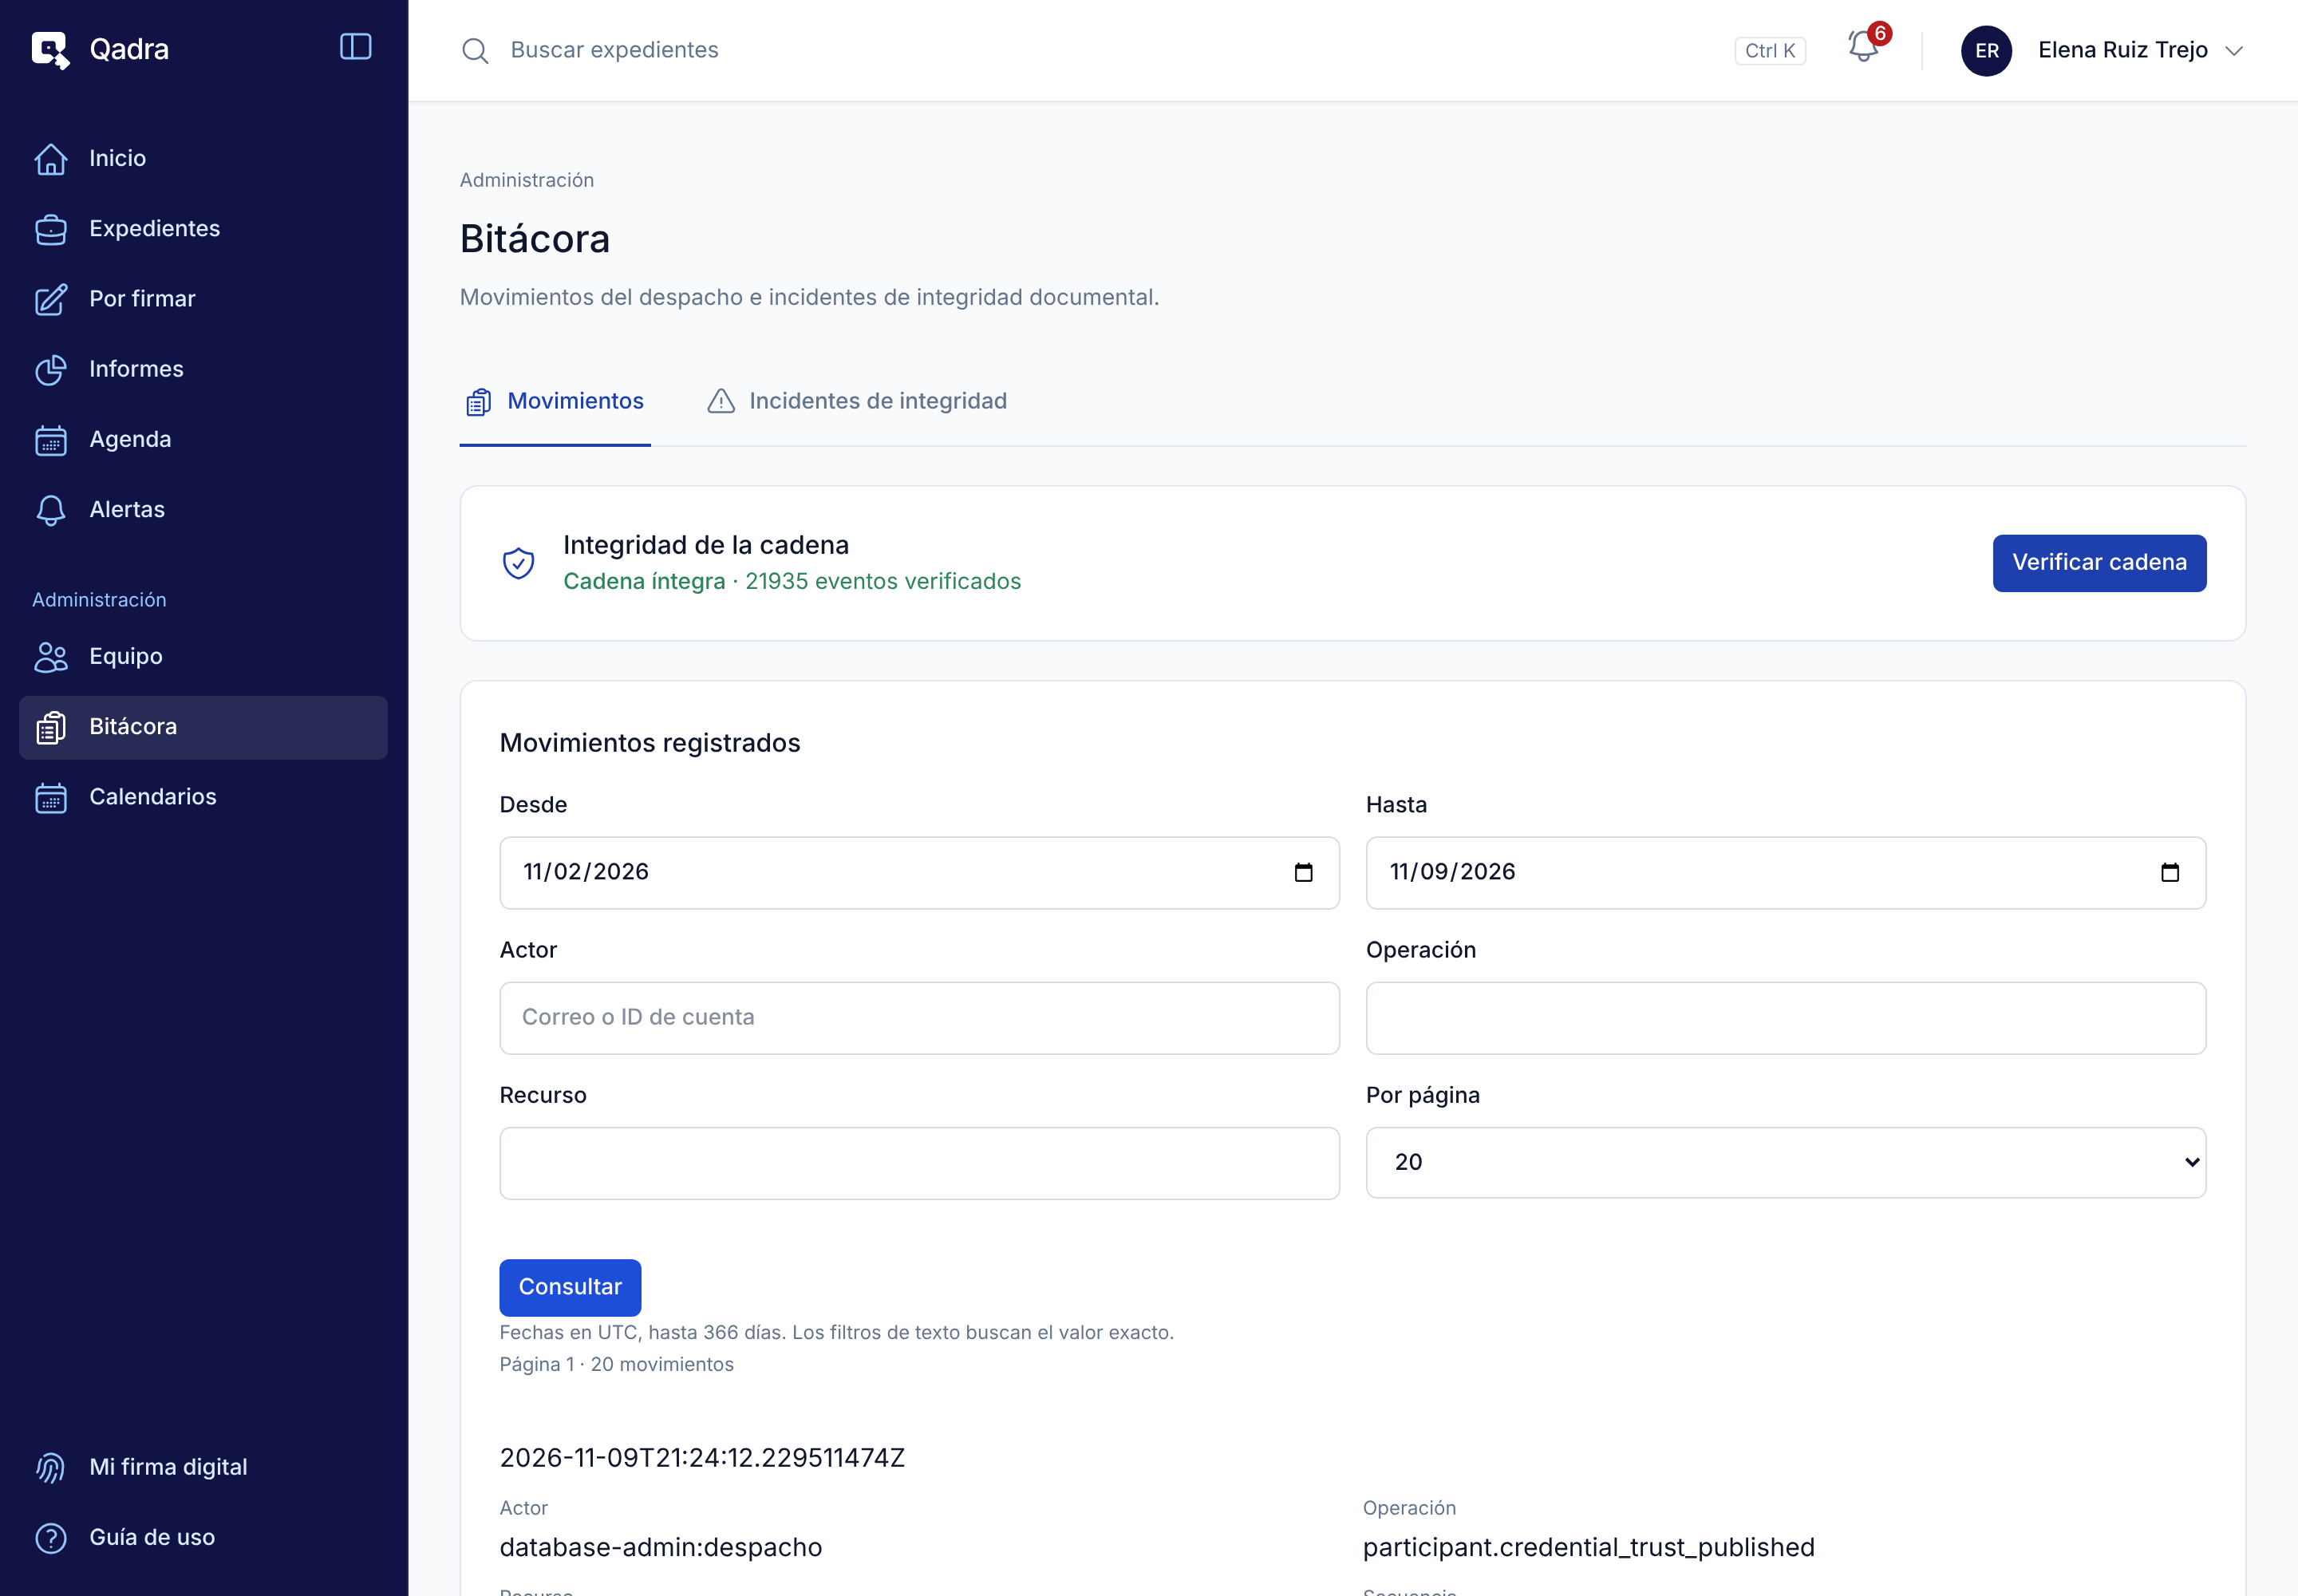
\includegraphics[width=0.9\textwidth]{capturas/A-48-bitacora.png}
  \caption{Bitácora del despacho.}
  \label{fig:manual-bitacora}
\end{figure}

\resultado Aparece \textbf{Cadena íntegra} con el número de eventos
verificados, y la lista de movimientos del periodo.

\importante{Si aparece \textbf{Alteración detectada}, la bitácora fue
modificada fuera de Qadra. Conserve el resultado y revise el primer evento
roto antes de cualquier otra acción. Si aparece el aviso \enquote{Hay
incidentes de integridad registrados.}, haga clic en
\textbf{Consultar incidentes}: un incidente no indica su causa ni a un
responsable.}

\nota{Las fechas de la bitácora están en UTC y el periodo máximo es de 366
días. Los filtros de texto buscan el valor exacto.}

% ---------------------------------------------------------------------
\section{Calendarios jurisdiccionales}\label{sec:calendarios}

\paraque Publica los días hábiles e inhábiles de cada autoridad, que Qadra
usa para calcular plazos.

\disponible Administrador (publica, reemplaza y retira). El Litigante y el
Asistente legal los consultan desde la \textbf{Agenda}.

\pasos\ Publicar un calendario:
\begin{enumerate}
  \item En el menú, haga clic en \textbf{Calendarios} y luego en
        \textbf{Publicar calendario}.
  \item Llene el \textbf{Ámbito declarado}: título, fuero, autoridad, órgano,
        territorio y entidades.
  \item Indique la \textbf{Cobertura civil} (hasta 1096 días) y el
        \textbf{Patrón semanal expreso} de cada día.
  \item Agregue las fechas inhábiles en \textbf{Excepciones por intervalo}
        y las referencias en \textbf{Fuentes públicas declaradas}.
  \item Haga clic en \textbf{Revisar calendario} y luego en
        \textbf{Confirmar calendario}.
\end{enumerate}

\begin{figure}[H]
  \centering
  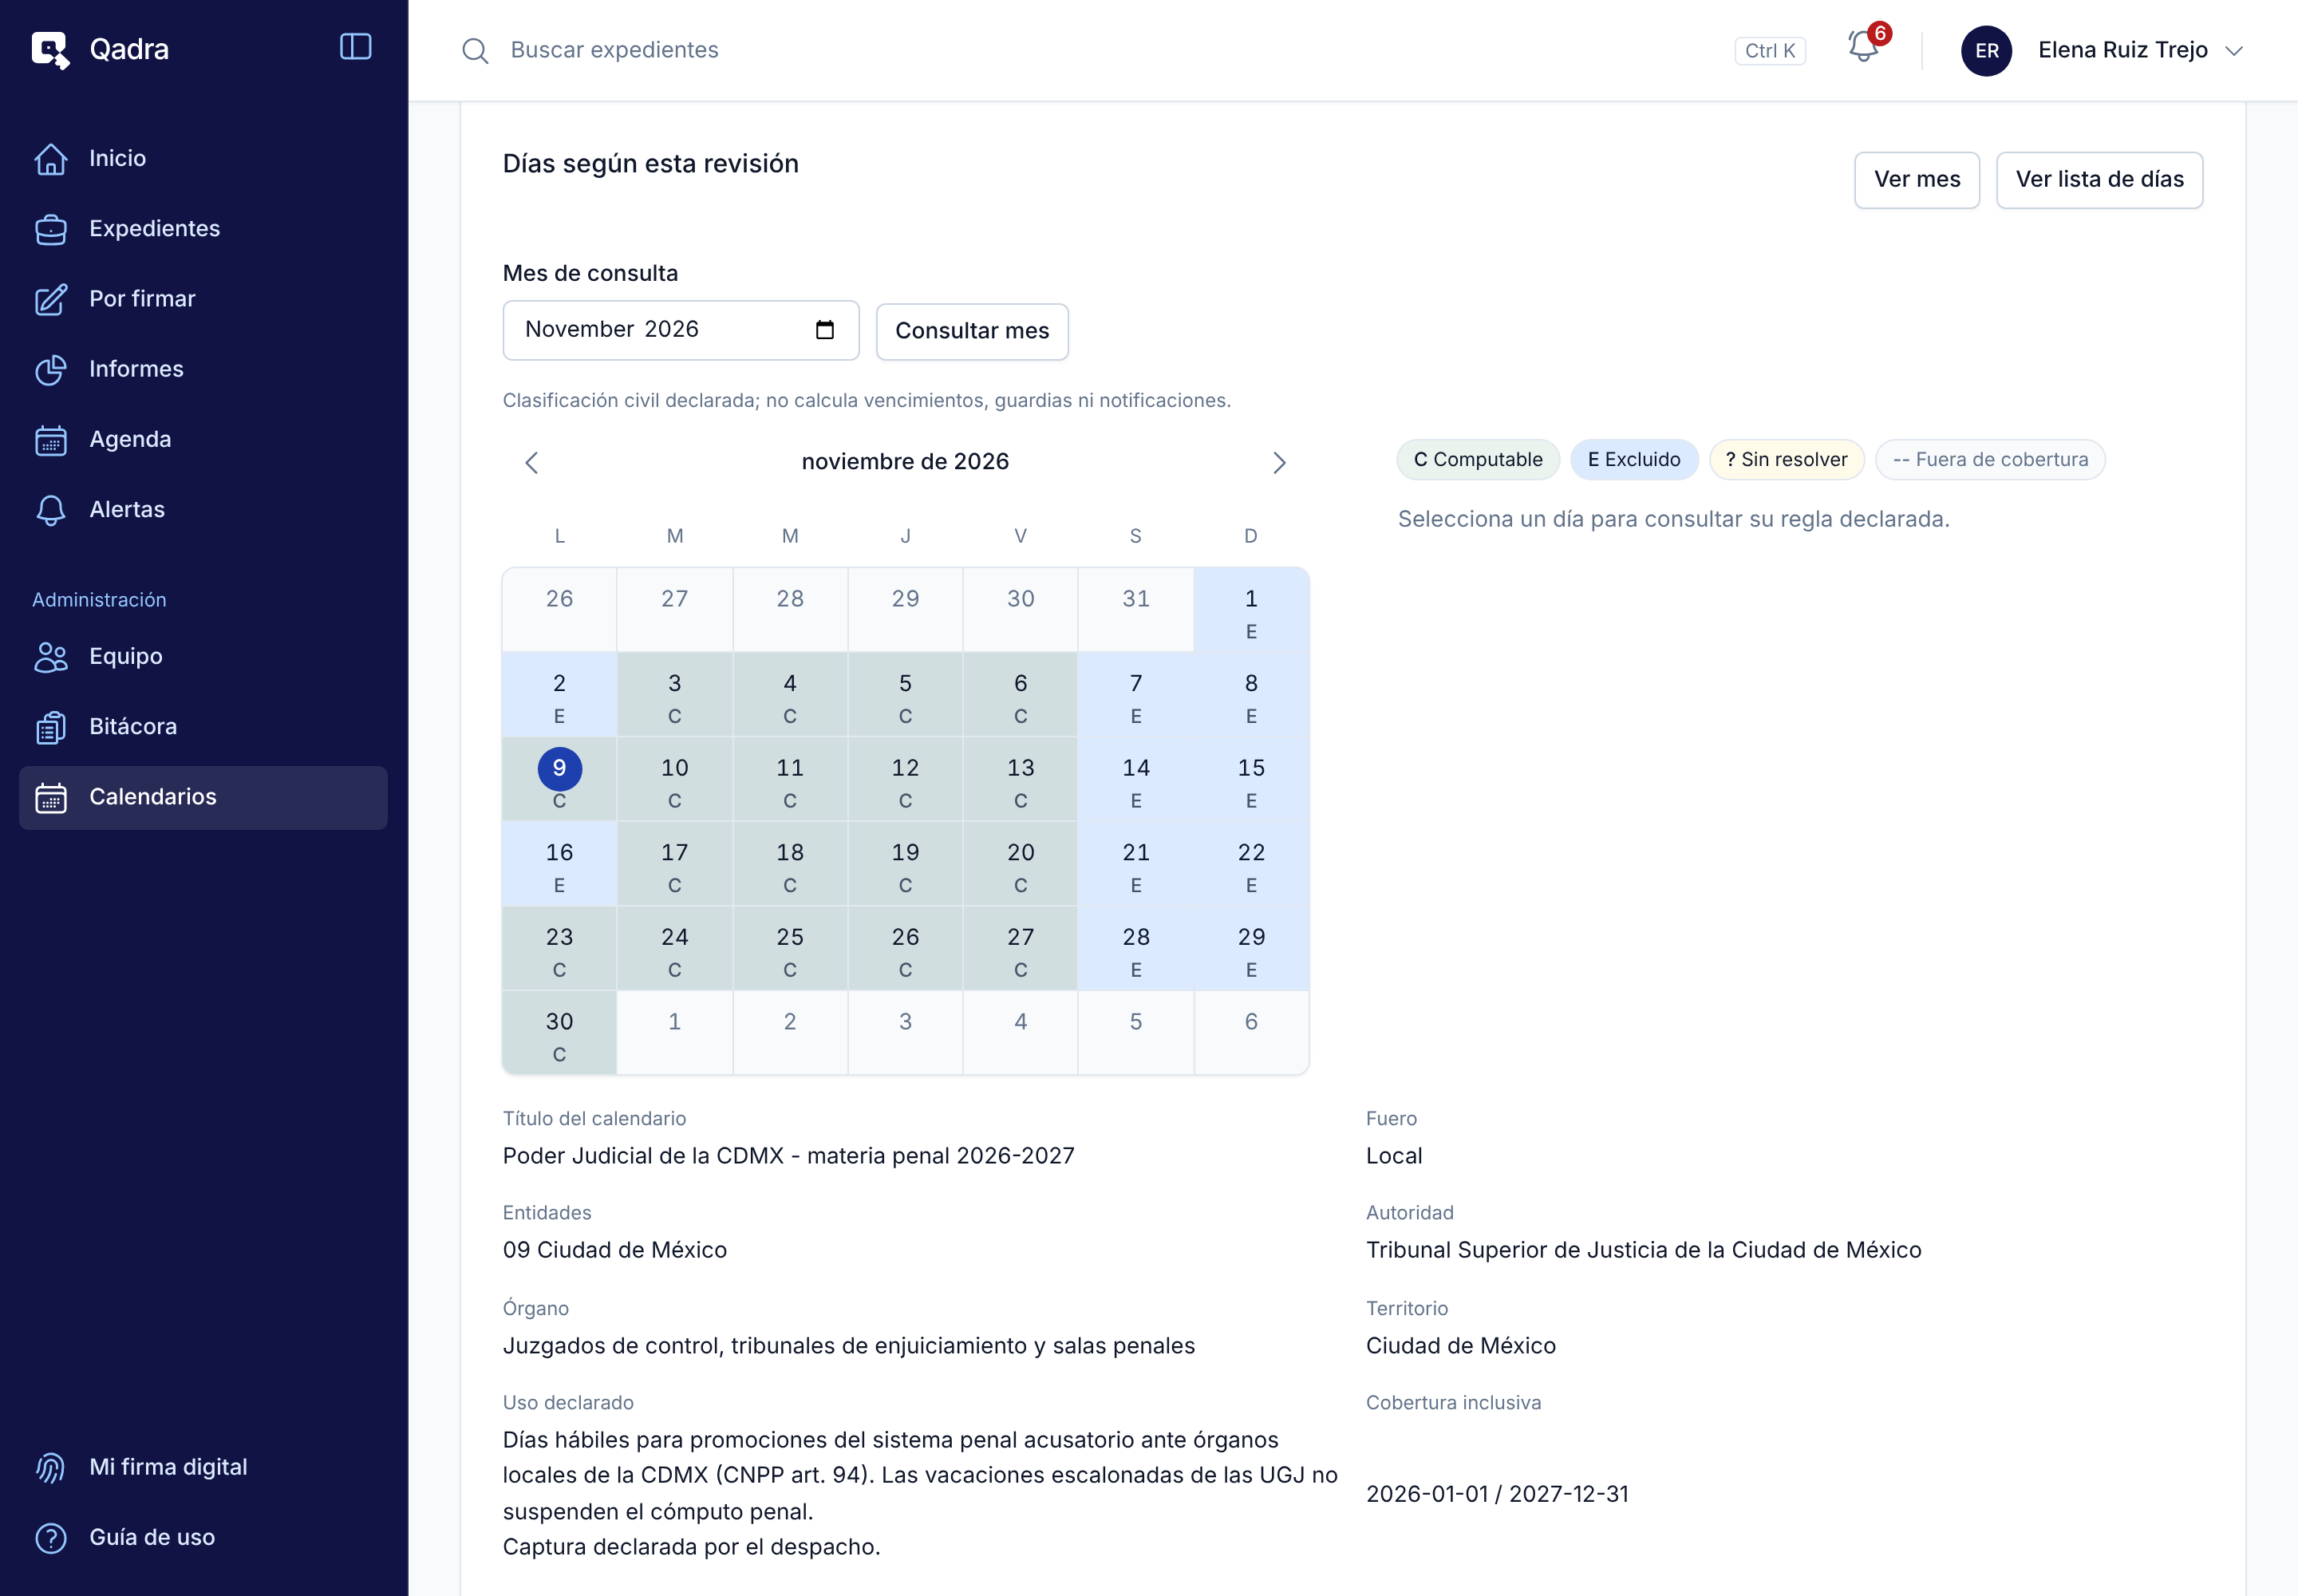
\includegraphics[width=0.9\textwidth]{capturas/A-49-calendarios.png}
  \caption{Calendarios jurisdiccionales.}
  \label{fig:manual-calendarios}
\end{figure}

\resultado Aparece \enquote{Calendario guardado con revisión y recibo.}

\begin{itemize}
  \item Para corregirlo, haga clic en \textbf{Reemplazar calendario} e
        indique el \textbf{Motivo}; la versión anterior queda en el historial.
  \item Para consultar cómo clasifica cada día, abra
        \textbf{Consultar calendario} y revise
        \textbf{Días según esta revisión}.
\end{itemize}

\importante{\textbf{Retirar calendario} es definitivo. Los plazos ya
calculados conservan su historial, pero el calendario no podrá usarse en
cálculos nuevos.}
